

\subsection{Skin friction drag}

Skin friction is one of the most notable sources of model rocket
drag.  It is caused by the friction of the viscous flow of air
around the rocket.  In his thesis Barrowman presented formulae for
estimating the skin friction coefficient for both laminar and
turbulent boundary layers as well as the transition between the
two~\cite[pp.~43--47]{barrowman-thesis}.  As discussed above, a fully
turbulent boundary layer will be assumed in this thesis.

%Two calculation methods will
%be presented, one for ``typical'' rockets and one for those with very
%fine precision finish.

The skin friction coefficient $C_f$ is defined as the drag coefficient
due to friction with the reference area being the total wetted area
of the rocket, that is, the body and fin area in contact with the
airflow:
%
\begin{equation}
C_f = \frac{D_{\rm friction}}{\frac{1}{2} \rho v_0^2\;A_{\rm wet}}
\end{equation}
%
The coefficient is a function of the rocket's Reynolds number $R$ and
the surface roughness.
%, defined
%as
%
%\begin{equation}
%R = \frac{v_0\;L_r}{\nu}
%\end{equation}
%
%where $v_0$ is the free-stream velocity of the rocket, $L_r$ is the
%length of the rocket and $\nu$ is the local kinematic viscosity of
%air.  
The aim is to first calculate the skin friction coefficient,
then apply corrections due to compressibility and geometry effects,
and finally to convert the coefficient to the proper reference area.


\subsubsection{Skin friction coefficients}
\label{sec-skin-friction-coefficient}

The values for $C_f$ are given by different formulae depending on the
Reynolds number.  If $R<5\cdot10^5$ the flow is assumed to be
completely laminar, and the corresponding skin friction coefficient is
%
\begin{equation}
C_f = \frac{1.328}{\sqrt{R}}.
\label{eq-laminar-friction}
\end{equation}
%
Correspondingly, for completely turbulent flow (also for low Reynolds
numbers when forced by some protrusion from the surface) the
coefficient is given by
%
\begin{equation}
C_f = \frac{1}{(1.50\; \ln R - 5.6)^2}.
\label{eq-turbulent-friction}
\end{equation}
%
Above $R=5\cdot10^5$ some of the flow around the rocket is turbulent
and some laminar.  Measured data of the transition results in an
empirical formula for the transition from
equation~(\ref{eq-laminar-friction}) to
equation~(\ref{eq-turbulent-friction}) as
%
\begin{equation}
C_f = \frac{1}{(1.50\;\ln R - 5.6)^2} - \frac{1700}{R}.
\label{eq-transition-friction}
\end{equation}
%
This equation gives a continuation from the laminar equation.  The
exact point of switch to the transitional equation is the point where
equations (\ref{eq-laminar-friction}) and
(\ref{eq-transition-friction}) are equal, $R=5.39\cdot10^5$.

% Exact transition point from laminar to transitional
%    R = 539154


The above formulae assume that the surface is ``smooth'' and the
surface roughness is completely submerged in a laminar sublayer.  At
sufficient speeds even slight roughness may have an effect on the skin
friction.  The critical Reynolds number corresponding to the roughness
is given by
%
\begin{equation}
R_{\rm crit} = 51\left(\frac{R_s}{L_r}\right)^{-1.039},
\end{equation}
%
where $R_s$ is an approximate roughess height of the surface.  A few
typical roughness heights are presented in Table~\ref{tab-roughnesses}.
For Reynolds numbers above the critical value, the skin friction
coefficient can be considered independent of Reynolds number, and has
a value of
%
\begin{equation}
C_f = 0.032\left(\frac{R_s}{L_r}\right)^{0.2}.
\label{eq-critical-friction}
\end{equation}
%

% TODO: ep�jatkuvuus karkeudessa
% mit� jos karkeus suurta?
% Katso Hoernerista!!


\begin{table}
\caption{Approximate roughness heights of different
  surfaces~\cite[p.~XXX]{hoerner}}
\label{tab-roughnesses}
\begin{center}
\begin{tabular}{lc}
Type of surface & Height / \um \\
\hline
Average glass                  & 0.1 \\
Finished and polished surface  & 0.5 \\
Optimum paint-sprayed surface  & 5 \\
Planed wooden boards           & 15 \\
% planed = h�yl�tty ???
Paint in aircraft mass production & 20 \\
Smooth cement surface          & 50 \\
Dip-galvanized metal surface   & 150 \\
Incorrectly sprayed aircraft paint & 200 \\
Raw wooden boards              & 500 \\
Average concrete surface       & 1000 \\
\hline
\end{tabular}
\end{center}
\end{table}


Finally, a correction must be made for very low Reynolds numbers.  The
experimental formulae are applicable above approximately
$R\approx10^4$.  This corresponds to velocities typically below 1~m/s,
and have therefore negligible effect on simulations.  Below this
Reynolds number, the skin friction coeffifient is assumed to be equal
as for $R=10^4$.


As a summary, when assuming the rocket to be finished with enough
precision to have a significant portion of laminar flow, the value of
$C_f$ is computed by
%
\begin{equation}
C_f = \left\{
\begin{array}{ll}
1.33\cdot10^{-2}, & \mbox{if $R<10^4$} \\
\mbox{Eq.~(\ref{eq-laminar-friction})}, & \mbox{if $10^4<R<5.39\cdot10^5$} \\
\mbox{Eq.~(\ref{eq-transition-friction})}, & \mbox{if 
      $5.39\cdot10^5 < R < R_{\rm crit}$} \\
\mbox{Eq.~(\ref{eq-critical-friction})}, & \mbox{if $R>R_{\rm crit}$}
\end{array}
\right. .
\end{equation}
%
When assuming a fully turbulent flow, $C_f$ is computed by
%
\begin{equation}
C_f = \left\{
\begin{array}{ll}
1.48\cdot10^{-2}, & \mbox{if $R<10^4$} \\
\mbox{Eq.~(\ref{eq-turbulent-friction})}, & \mbox{if $10^4<R<R_{\rm crit}$} \\
\mbox{Eq.~(\ref{eq-critical-friction})}, & \mbox{if $R>R_{\rm crit}$}
\end{array}
\right. .
\end{equation}
%
These formulae are plotted in Figure~\ref{fig-skinfriction-plot}.

\begin{figure}
\centering
\epsfig{file=figures/drag/skinfriction.eps,width=11cm}
\caption{Skin friction coefficient of fully laminar
  (Eq.~(\ref{eq-laminar-friction})), fully turbulent
  (Eq.~(\ref{eq-turbulent-friction})), transitional
  (Eq.~(\ref{eq-transition-friction})) and roughness-limited
  (Eq.~(\ref{eq-critical-friction})) boundary layers.}
\label{fig-skinfriction-plot}
% TODO: kuva matlabilla, kapeampi pystysuunnassa
\end{figure}


\subsubsection{Compressibility corrections}

The laminar skin friction coefficient is constant at both subsonic and
low supersonic speeds, ${C_f}_c = C_f$.  However, at subsonic speeds
the smooth turbulent value of equation~(\ref{eq-turbulent-friction})
and the roughness-limited value of
equation~(\ref{eq-critical-friction}) must be corrected with
%
\begin{equation}
{C_f}_c = C_f\; (1-0.1\, M^2).
\end{equation}
%
In supersonic flow, the smooth turbulent skin friction coefficient
must be corrected with
%
\begin{equation}
{C_f}_c = \frac{C_f}{(1+0.15\, M^2)^{0.58}}
\end{equation}
%
and the roughness-limited value with
%
\begin{equation}
{C_f}_c = \frac{C_f}{1 + 0.18\, M^2}.
\end{equation}
%
However, the corrected roughness-limited value should not be used if
it would yield a value smaller than the corresponding smooth turbulent
value.  In order not to cause discontinuities, the transition point
from of laminar to turbulent corrections and from subsonic to
supersonic is done gradually over a suitable Reynolds number or Mach
number range.



\subsubsection{Skin friction drag coefficient}
\label{sec-skin-friction-drag}

After correcting the skin friction coefficient for compressibility
effects, the coefficient can be converted into the actual drag
coefficient.  This is performed by scaling it to the correct reference
area.  The body wetted area is corrected for its cylindrical geometry,
and the effect of finite fin thickness which Barrowman handled
separately is also included~\cite[p.~55]{barrowman-thesis}.  The total
friction drag coefficient is then
%
\begin{equation}
(C_D)_{\rm friction} = {C_f}_c \; \frac{
  \del{1 + \frac{1}{2f_B}} \cdot A_{\rm wet,body} + 
  \del{1 + \frac{2t}{\bar c}} \cdot A_{\rm wet,fins}}
   {\Aref}
\label{eq-friction-drag-scale}
\end{equation}
%
where $f_B$ is the fineness ratio of the rocket, and $t$ the thickness
and $\bar c$ the mean aerodynamic chord length of the fins.  The
wetted area of the fins $A_{\rm wet,fins}$ includes both sides of the
fins.


